Als we de + en de - van een batterij met elkaar verbinden dat maken we een kortsluiting. Bij een kortsluiting gaat er heel veel stroom lopen, zoveel zelfs dat het plastic om de geleider in brand zou kunnen vliegen. Om te voorkomen dat dat gebeurd moeten we de stroom beperken. Dit doen we door de weerstand\index{Weerstand} te verhogen. De weerstand vermindert de stroom en daardoor ontstaat er geen brand.

Er zijn verschillende manieren om de weerstand te verhogen. We kunnen gebruik maken van een apparaat dat de stroom gebruikt om te werken (bijvoorbeeld een lamp die brandt), maar we kunnen ook een speciaal stukje elektronica gebruiken, genaamd een weerstand\index{Weerstand}\index{Resistor} die als enige functie heeft de weerstand in een circuit te verhogen zodat de stroom beperkt wordt.

In de elektronica wordt een weerstand weergegeven met het symbool dat je ziet weergegeven in \ref{symbool:weerstand}

\begin{figure}[h]
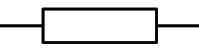
\includegraphics[width=5cm]{weerstand}
\centering
\caption{Symbool van een weerstand}
\label{symbool:weerstand}
\end{figure}

